   \documentclass{beamer}
%
% Choose how your presentation looks.
%
% For more themes, color themes and font themes, see:
% http://deic.uab.es/~iblanes/beamer_gallery/index_by_theme.html
%
\mode<presentation>
{
  \usetheme{Boadilla}     % or try Boadilla, Darmstadt, Madrid, Warsaw, default, ...
  \usecolortheme{default} % or try Boadilla, albatross, beaver, crane, default, ...
  \usefonttheme{default}  % or try Boadilla, serif, structurebold, default, ...
  \setbeamertemplate{navigation symbols}{}
  \setbeamertemplate{caption}[numbered]
} 

\usepackage[english]{babel}
\usepackage[utf8x]{inputenc}
\usepackage{caption}
\usepackage{subcaption}
\newenvironment{variableblock}[3]{%
  \setbeamercolor{block body}{#2}
  \setbeamercolor{block title}{#3}
  \begin{block}{#1}}{\end{block}}
\title[]{Optical Isolation with Nonlinear Topological Photonics}
%\author[CDTec] {Cristian Pereira, André Einhardt, Mateus Nascimento}
\author[] {Xin Zhou, You Wang, Daniel Leykam and Yidong Chong}

\institute[]{Nanyang Technological University, Singapore}
\date{September 2017}


\begin{document}

\begin{frame}
    \begin{center}
  \titlepage 
      \begin{figure}[h]
  
\includegraphics[width=2.3cm,height=2.3cm] {/home/zhouxin/research/conference/presentation/mtheme/slides/icon.png}
  \hspace*{3.0em}
  
\includegraphics[width=3.5cm,height=2.1cm,scale=1] {/home/zhouxin/research/conference/presentation/mtheme/slides/ntu_logo.png}
      \end{figure}
  \end{center}
\end{frame}

% Uncomment these lines for an automatically generated outline.
%\begin{frame}{Outline}
%  \tableofcontents
%\end{frame}

\section{Outline}
\begin{frame}{Outline}
    \begin{itemize}
      \item Optical Isolation
      \begin{itemize}
      \item What is optical isolator
      \item Why we want optical isolator
      \item How to achieve optical isolation
      \end{itemize}
      \item Topological Photonics
            \begin{itemize}
            \item Topological state
            \item Realizing Topological Edge State in Photonic System
		    \end{itemize}
      
      \item Topological Optical Isolation 
            \begin{itemize}
            \item 1D SSH model
            \item 2D Haldane model
            \item 2D lattice of coupled ring waveguides
		    \end{itemize}
	  \end{itemize}        
  \vskip 5cm
\end{frame}

\section{Optical Isolation}
% ================== ÁREAS SENDO ALTERADAS POR CRISTIAN PEREIRA ==================
\begin{frame}{What is Optical Isolation}
Optical isolators are devices that allow light to pass in one direction (e.g., along a waveguide), while blocking transmission in the other direction, thus acting as the analogues of diodes in electronic circuits
\begin{figure}

  \centering
    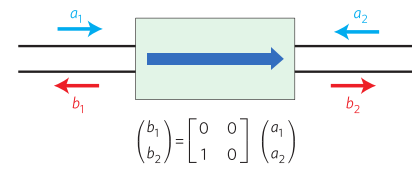
\includegraphics[width=0.5\textwidth]{/home/zhouxin/research/conference/presentation/mtheme/slides/isolator.png}
      \caption{A schematic picture of optical isolator.}
\end{figure}
     \vskip -0.5cm
    \begin{block}
    {Why we need it}
      \begin{itemize}
        \item In modern fibre communication networks it is an essential device to prevent interference between different parts of the networks.
        \item Nowadays people become more and more interested in large-scale on-chip optical networks, so optical isolation on-chip size is becoming increasingly important.
    \end{itemize}
  \end{block}
\end{frame}

 


\begin{frame}{How to Achieve Optical Isolation}
     \vskip -0.15cm
    \begin{block}{Lorenz Reciprocity}

For linear, static and non-magnetic material,
     \vskip -0.75cm
\begin{equation}
\nabla \cdot (\textbf{$E^{'}$} \times\textbf{$H^{''}$} - \textbf{$E^{''}$} \times\textbf{$H^{'}$}) = j\omega(\textbf{$E^{''}$} \textbf{$\epsilon$} \textbf{$E^{'}$} - \textbf{$E^{'}$} \textbf{$\epsilon$} \textbf{$E^{''}$} - H^{''} \mu \textbf{$H^{'}$}+H^{'} \mu \textbf{$H^{''}$} ) = 0 
\end{equation}
     \vskip -0.25cm
Here, ($E^{'}, H^{'}$) and ($E^{''}, H^{''}$) are two sets of excitation.
  \end{block}
       \vskip -0.75cm
\begin{columns}[t]
  \begin{column}{0.325\textwidth}
    \begin{block}{Magneto-Optical Effect}
For magneto-optical material so $\epsilon$ and $\mu$ are non-symmetric tensor.
     \vskip -0.4cm
  \begin{figure}
    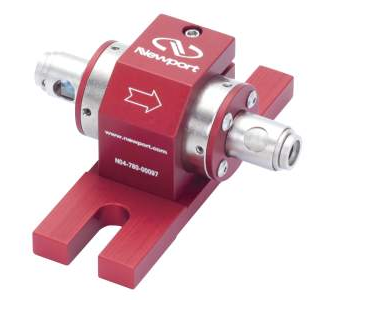
\includegraphics[width=3cm,height=2cm] {/home/zhouxin/research/conference/presentation/mtheme/slides/isolator_faraday.png}


  \end{figure}
    \end{block}
  \end{column}
  \begin{column}{0.325\textwidth}
    \begin{block}{Optical Nonlinear Material}
      For nonlinear material,$\epsilon$ and $\mu$ depend on $E$ and $H$
   \vskip -0.85cm
  \begin{figure}

    \includegraphics[width=4cm,height=2.5cm] {/home/zhouxin/research/conference/presentation/mtheme/slides/pt_isolator.pdf}
         \vskip -0.4cm
     \end{figure}
    \end{block}
  \end{column}
  \begin{column}{0.325\textwidth}
    \begin{block}{Spacial-temporal Modulation}
      For $\epsilon$ and $\mu$ depend on time, the derivation is not valid, so does Lorentz Reciprocity.
    \end{block}
  \end{column}

\end{columns}
\end{frame}



\begin{frame}{Topological Photonics}
 \vskip -0.1cm
\begin{block}{Realizing Topological State in Photonic System}

Photonic Crystal  \hspace*{3.0em}   Photonic Waveguide \hspace*{3.0em}
Ring \hspace*{.1em} Resonator
     \vskip -.75cm
\begin{figure}
    \centering
    \begin{subfigure}[t]{0.3\textwidth}
        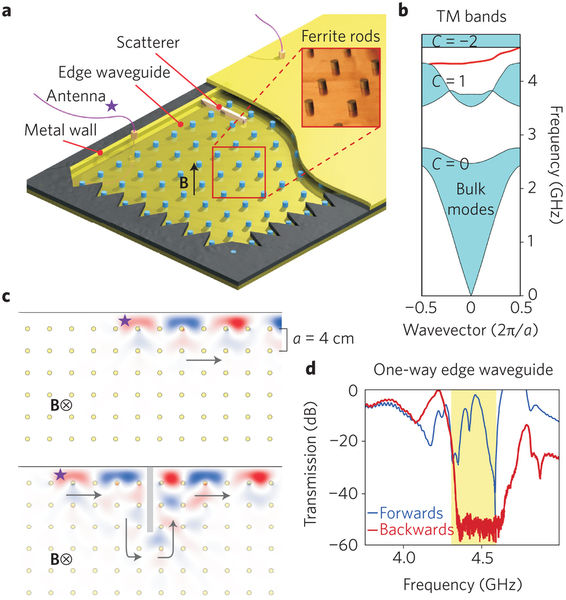
\includegraphics[width=\textwidth]{/home/zhouxin/research/conference/presentation/mtheme/slides/photonic_crystal.jpg}
        \vspace*{0.25cm}
     \caption*{{\tiny \mbox{Nature, 461(7265), 772-5(2009).}}}
        \label{fig:gull}
    \end{subfigure}\hspace*{-.7em}%
    ~ %add desired spacing between images, e. g. ~, \quad, \qquad, \hfill etc. 
      %(or a blank line to force the subfigure onto a new line)
    \begin{subfigure}[t]{0.45\textwidth}
    \vspace*{-3.8555cm}
        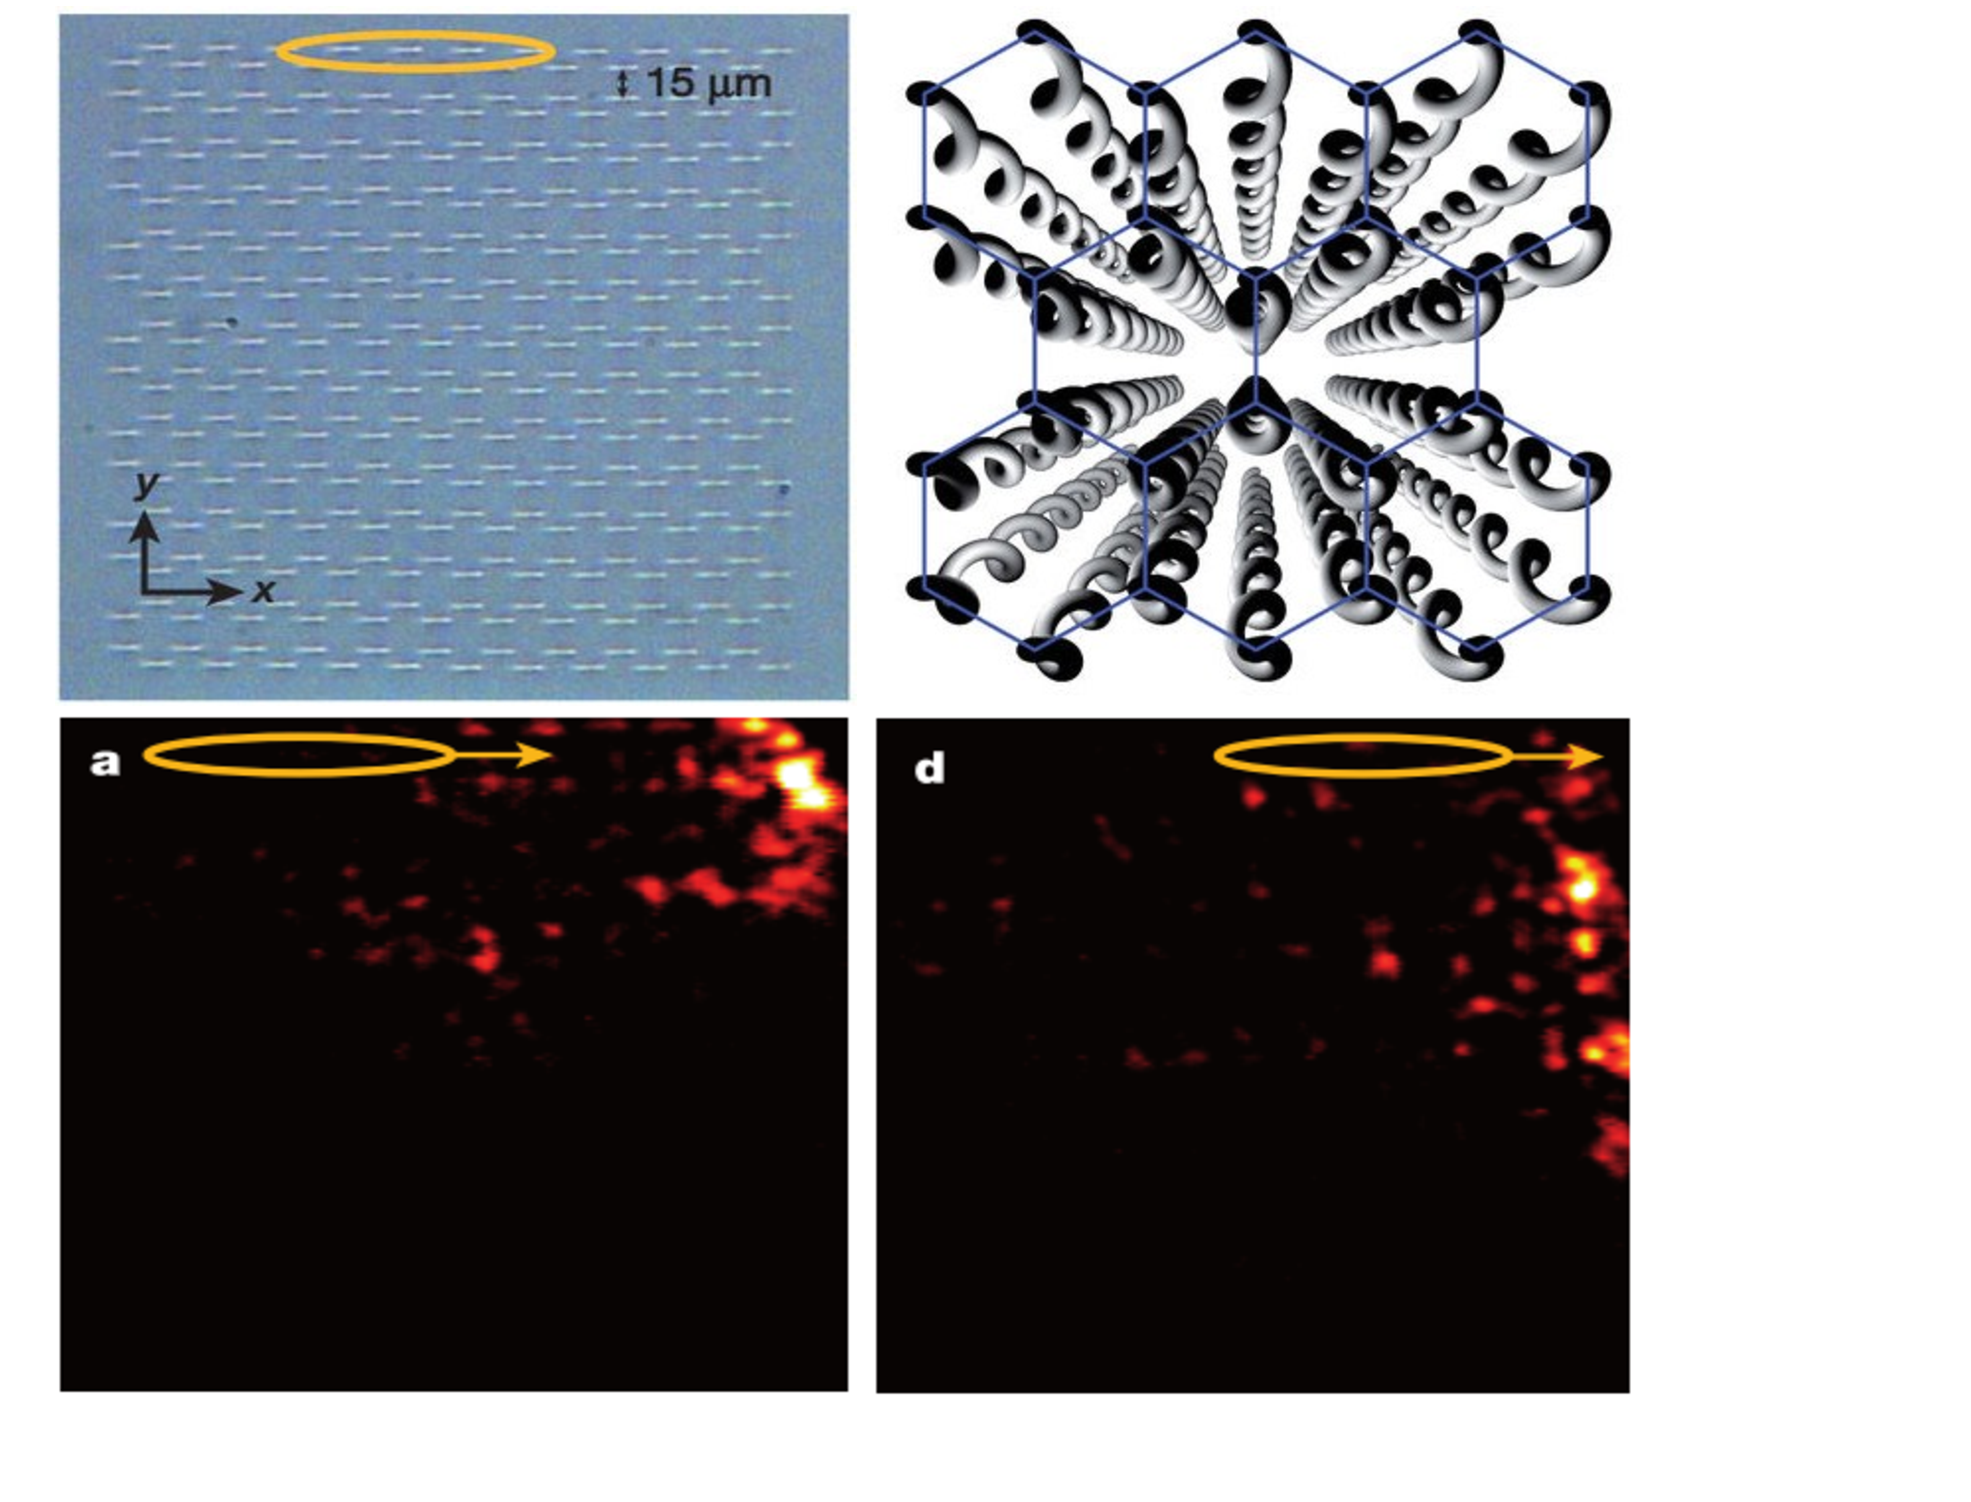
\includegraphics[width=\textwidth, height=0.7575\textwidth]{/home/zhouxin/research/conference/presentation/mtheme/slides/waveguide.pdf}
     \caption*{{\tiny Nature Photon. 7, 153–158 (2013).}}
        \label{fig:tiger}
    \end{subfigure}\hspace*{-3.7em}%
        \begin{subfigure}[t]{0.45\textwidth}
            \vspace*{-3.9055cm}
        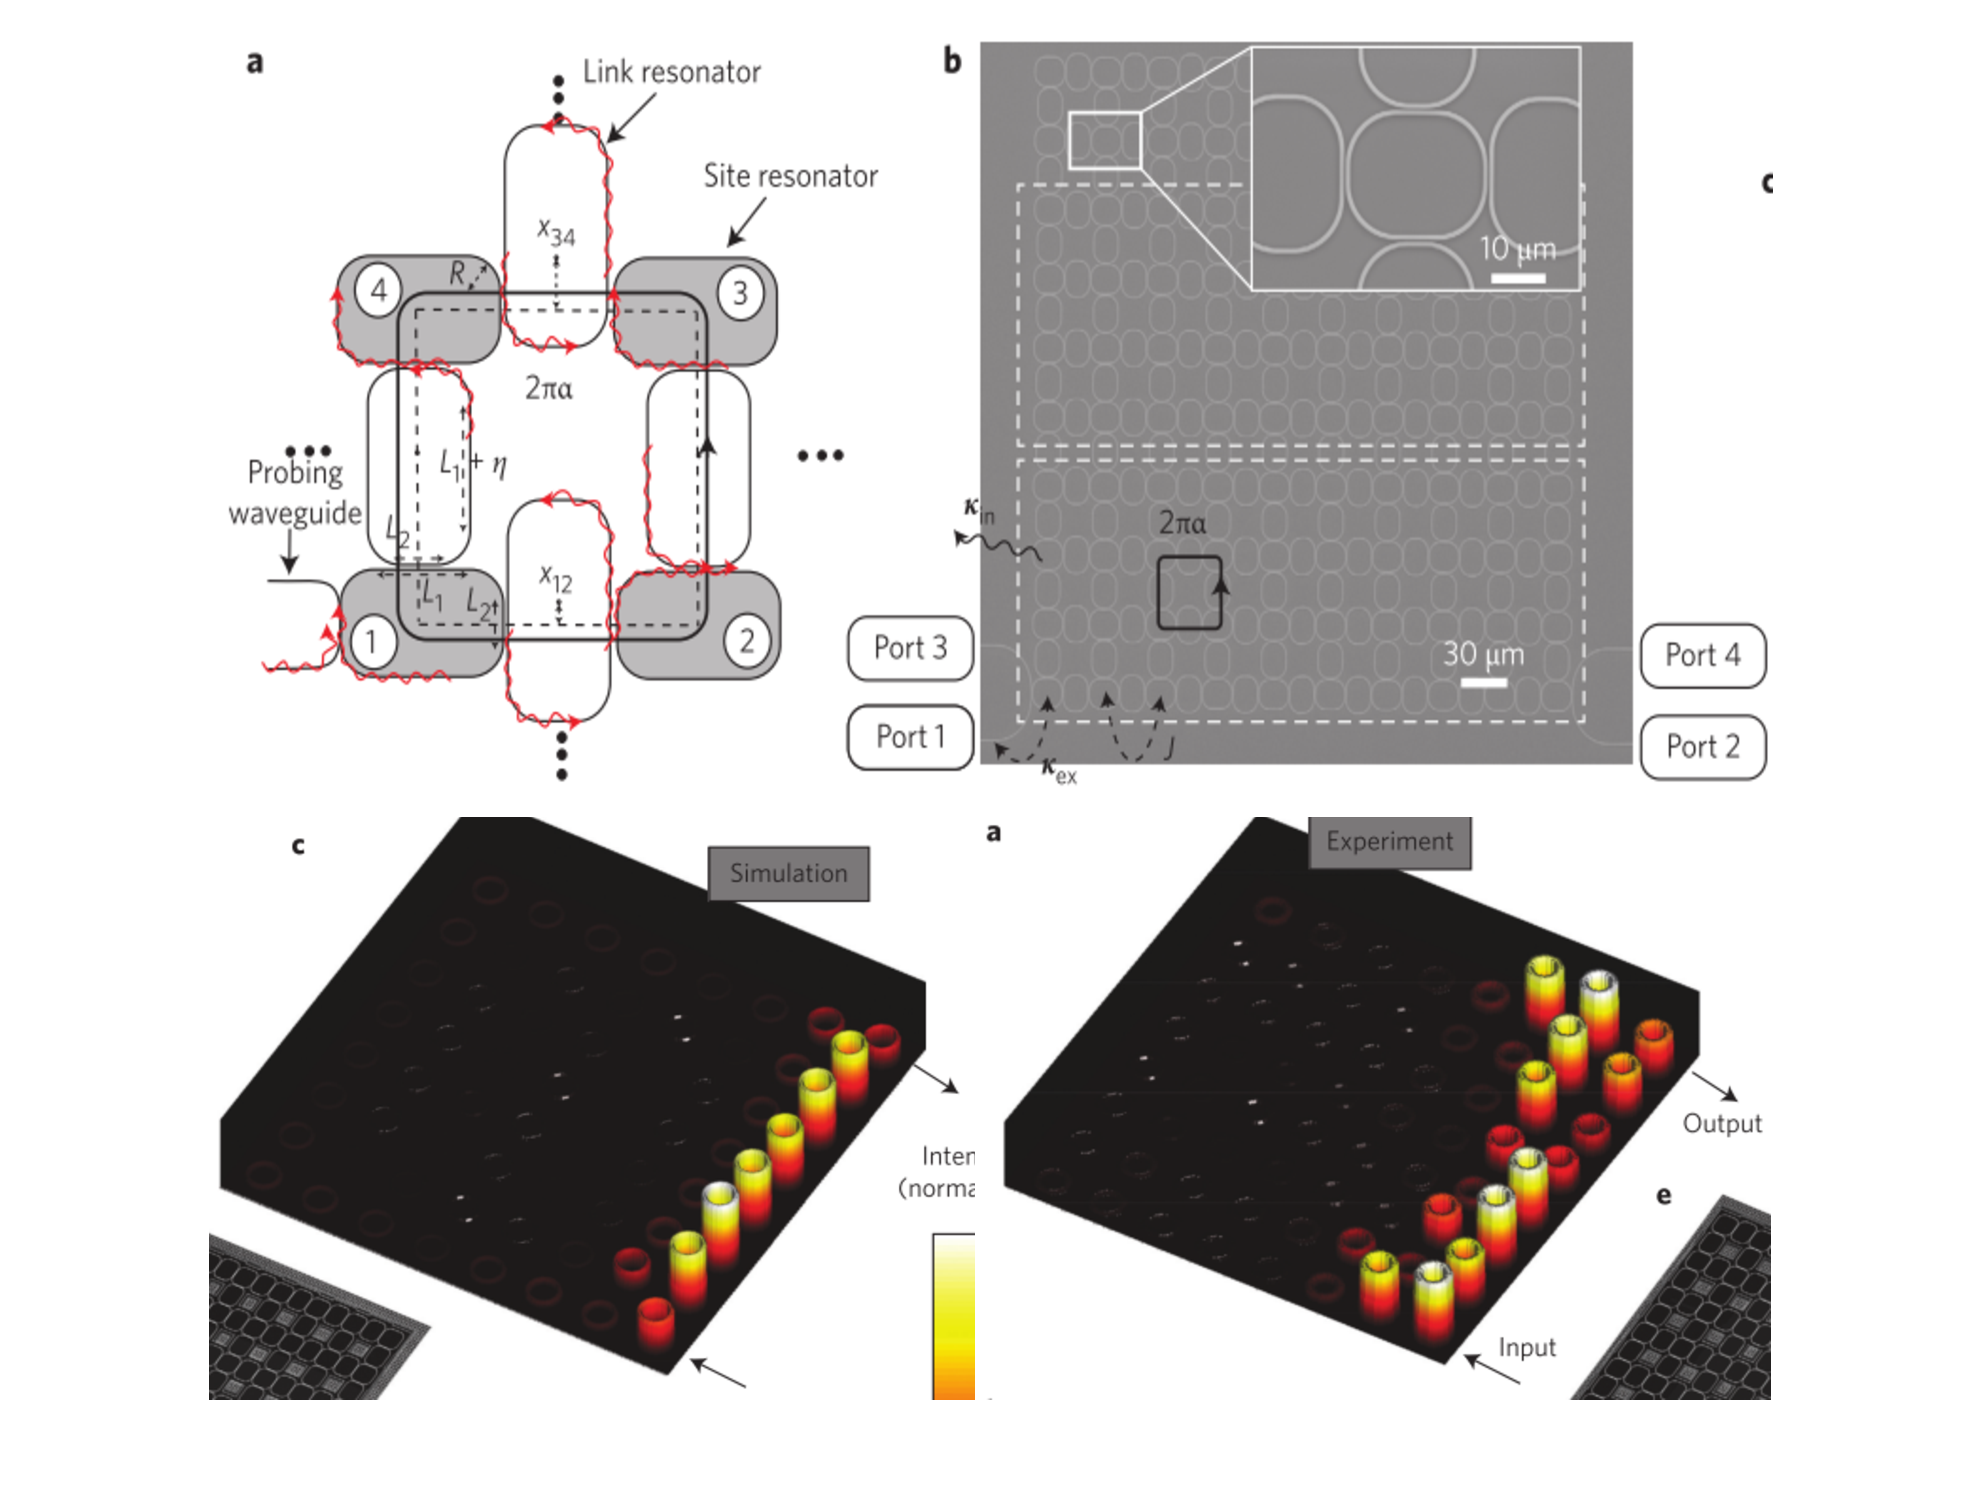
\includegraphics[width=0.9\textwidth, height=0.7675\textwidth]{/home/zhouxin/research/conference/presentation/mtheme/slides/resonator.pdf}
        \hspace*{-3.7em}
\caption*{{\tiny Nature Photon. 7, 1001–1005 (2013).}}
        \label{fig:gull}
    \end{subfigure}\hspace*{8.0em}
\label{fig:animals}
\end{figure}      

%\begin{variableblock}{Title}{bg=white}{bg=white}
%d
%\end{variableblock}

\end{block}
 \vspace*{-.5cm}
\begin{block}{Key Feature of Topological Edge State}
\begin{itemize}
\item Propagate along the edge without scattering into the bulk
\item Unidirectional without backscattering
\item Robust even in the presence of impurities
\end{itemize}
\end{block}


\end{frame}
% =================================== FIM MATEUS =================================

\begin{frame}{Topological Optical Isolation}
         \vskip -1.cm 
         \begin{block}{Nonlinear 1D Su–Schrieffer–Heeger (SSH) model}
         
       \begin{columns}
          \column{0.58\linewidth}
             %\centering
             \hspace*{0.5em}
             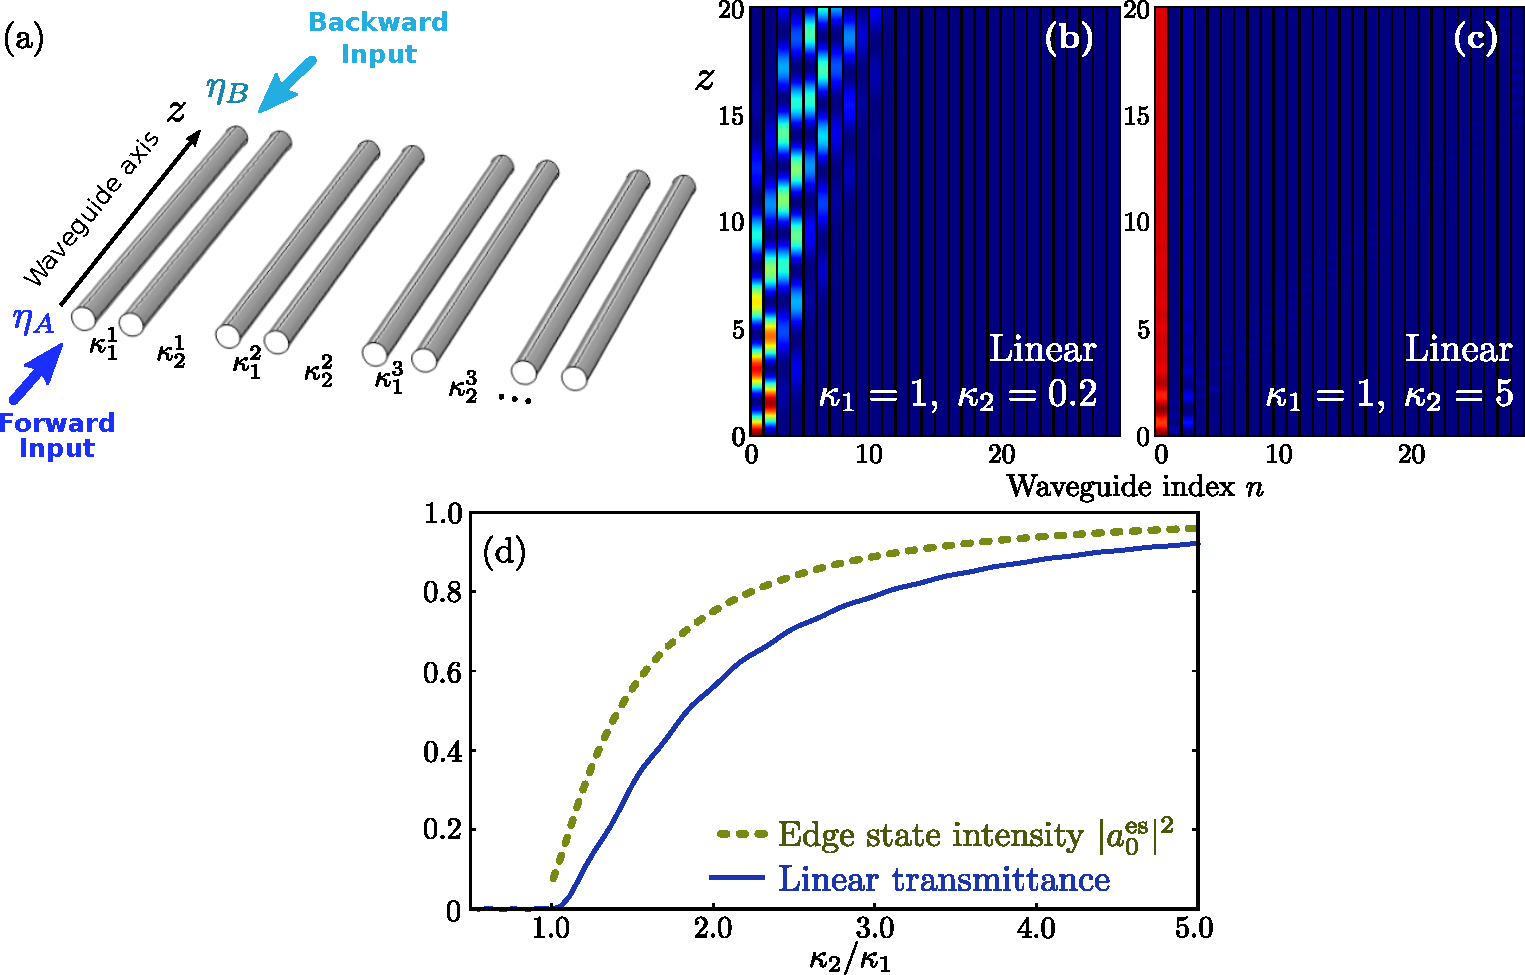
\includegraphics[width=0.9\textwidth, height=0.8\textwidth]{/home/zhouxin/research/conference/presentation/mtheme/slides/ssh.pdf}\hspace*{-10.5em}
           \column{0.4\linewidth}
                    \vskip -0.5cm 
Using coupled-mode theory:
\begin{eqnarray}
i\frac{da_n}{dz} = \kappa_{1}^{n}b_n + \kappa_{2}^{n-1}b_{n-1}\\
i\frac{db_n}{dz} = \kappa_{1}^{n}a_n + \kappa_{2}^{n-1}a_{n+1}	
\end{eqnarray}


\begin{itemize}
\item Topological transition at $\kappa_1$ = $\kappa_2$
\item Edge state with zero eigenvalue appear when $\kappa_1 < \kappa_2$ 
\end{itemize}


         \end{columns}
         \end{block}
\begin{block}{Transmittance}
\begin{equation}
\hspace*{-15.7em}
T = \frac{|a_{0}(Z)|^2}{I}, I = |a_{0}(0)|^2 
\end{equation}
I is input power and Z is pre-defined propagation distance.
\end{block}
\end{frame}




\begin{frame}{Topological Optical Isolation}
         \vskip -1.cm 
         \begin{block}{Nonlinear 1D Su–Schrieffer–Heeger (SSH) model}
Nonlinear coupling
\begin{equation}
\hspace*{-15.7em}
\kappa_{2}^{n}(z) = \kappa_0 + \alpha(|a_{n+1}(z)|^2|+b_{n}(z)|^2)
\end{equation}
$\kappa_1=1$, $\kappa_0=0.5$, $\alpha=1$, Z=20
\end{block}

 \vskip -0.3cm

         \begin{block}{}
         
       \begin{columns}
          \column{0.58\linewidth}
             %\centering
             \hspace*{0.5em}
             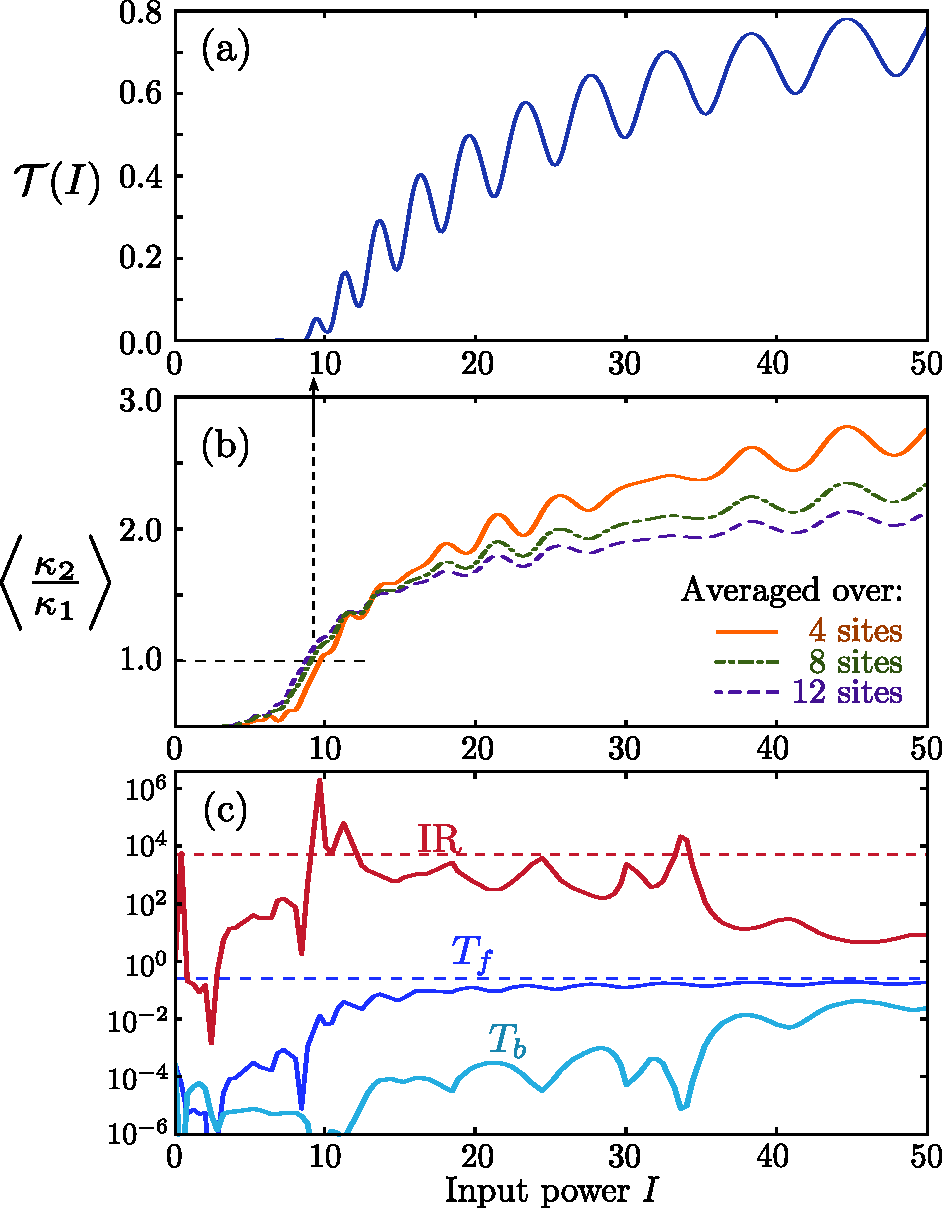
\includegraphics[width=0.9\textwidth, height=0.8\textwidth]{/home/zhouxin/research/conference/presentation/mtheme/slides/isolation.pdf}\hspace*{-10.5em}
           \column{0.4\linewidth}
                    \vskip -0.5cm 
 \vskip 0.1cm
Forward transmittance:
 \vskip -0.75cm
\begin{equation}
T_f=\eta_{A}^2\eta_{B}^2 T(\eta_{A}^2 I)
\end{equation}
 \vskip -.4cm
Backward transmittance:
 \vskip -0.75cm
\begin{equation}
T_b=\eta_{A}^2\eta_{B}^2 T(\eta_{B}^2 I)
\end{equation}
 \vskip -.2cm
Isolation Ratio:
 \vskip -0.5cm
\begin{equation}
IR=\frac{T_f}{T_b}
\end{equation}


 \vskip -0.1cm
 \hspace*{-2em}
{\small 1.T(I) increase significantly when $<\frac{\kappa_2}{\kappa_1}>$ crosses 1}

 \hspace*{-2em}
{\small 2.$<\frac{\kappa_2}{\kappa_1}>=1$ indicates topological trnasition for underline linear lattice}

 \hspace*{-2em}
{\small 3.$T_b$ is pretty smaller comparing to $T_f$ in a broad range of I}



         \end{columns}
         \end{block}

\end{frame}
\begin{frame}{Topological Optical Isolation}
         \vskip -1.cm 
         \begin{block}{Nonlinear 2D Haldane Model}       
       \begin{columns}
          \column{0.25\linewidth}
             %\centering
             \hspace*{-2em}
             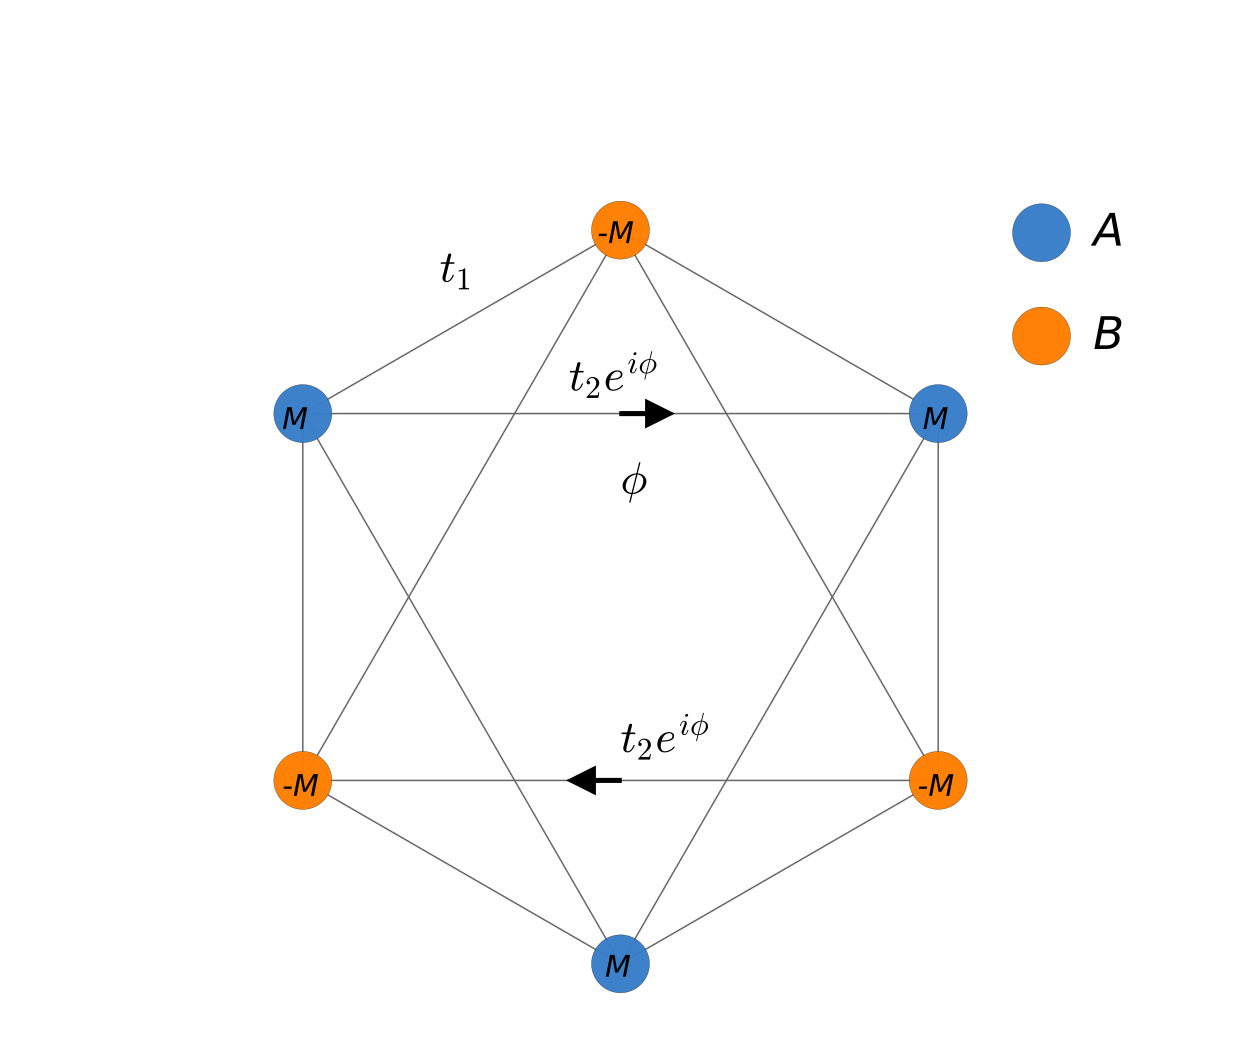
\includegraphics[width=1.0\textwidth, height=1.0\textwidth]{/home/zhouxin/research/conference/presentation/mtheme/slides/haldane_lattice.png}
             
          \column{0.25\linewidth}
             %\centering
             \hspace*{-5em}
             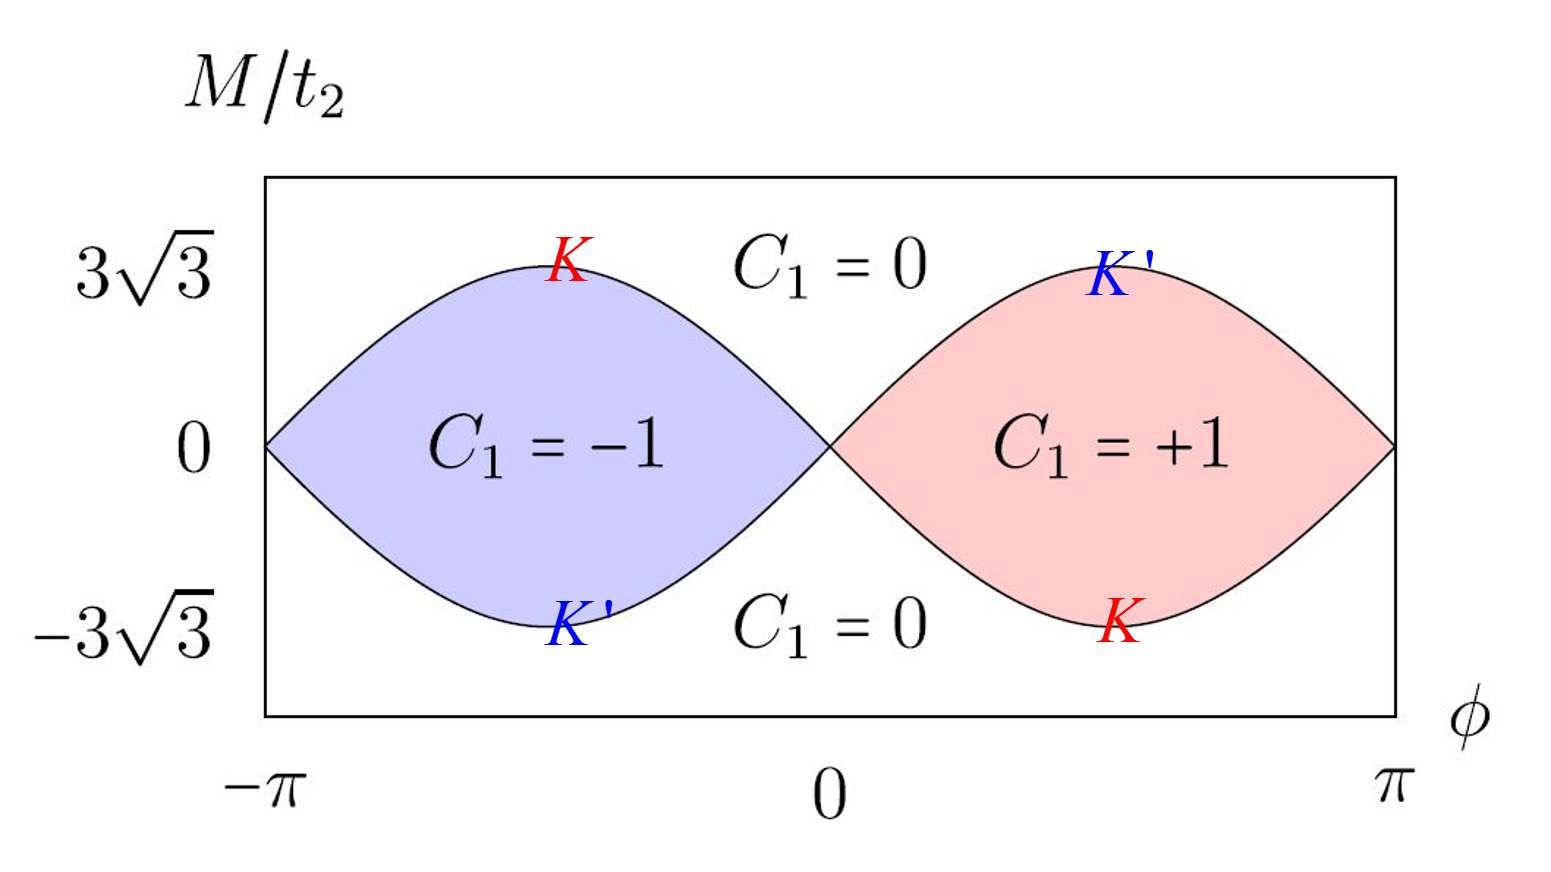
\includegraphics[width=1.0\textwidth, height=1.0\textwidth]{/home/zhouxin/research/conference/presentation/mtheme/slides/pd.png}\hspace*{-10.5em}             
             
             
           \column{0.2\linewidth}
                    \vskip -0.5cm 
\hspace*{-4.5em}
\mbox{Nonlinear on-site potential}
 \vskip 0.cm 

\hspace*{-6.5em}
$m_A^{\mu} = \frac{m_0}{1+|a_{\mu}|^2}, m_B^{\mu} = \frac{-m_0}{1+|b_{\mu}|^2}$
\hspace*{-6.5em}
\mbox{$t_1=1, t_2=\frac{1}{3}, \phi=\frac{\pi}{2}, m_0=2$}

\vskip 0.2cm
\hspace*{-6.5em}
\mbox{For fixed $t_1, t_2, \phi$, topological phase} 
\hspace*{-6.5em}
\mbox{ transition happens at} 
\hspace*{-4.5em}
\mbox{$m_A-m_B=|6\sqrt{3}t_2\sin{\phi}|$}
         \end{columns} 
         \end{block}

 \vskip -0.6cm
         \begin{block}{}
         
       \begin{columns}
          \column{0.55\linewidth}
             %\centering
             \hspace*{0.5em}
             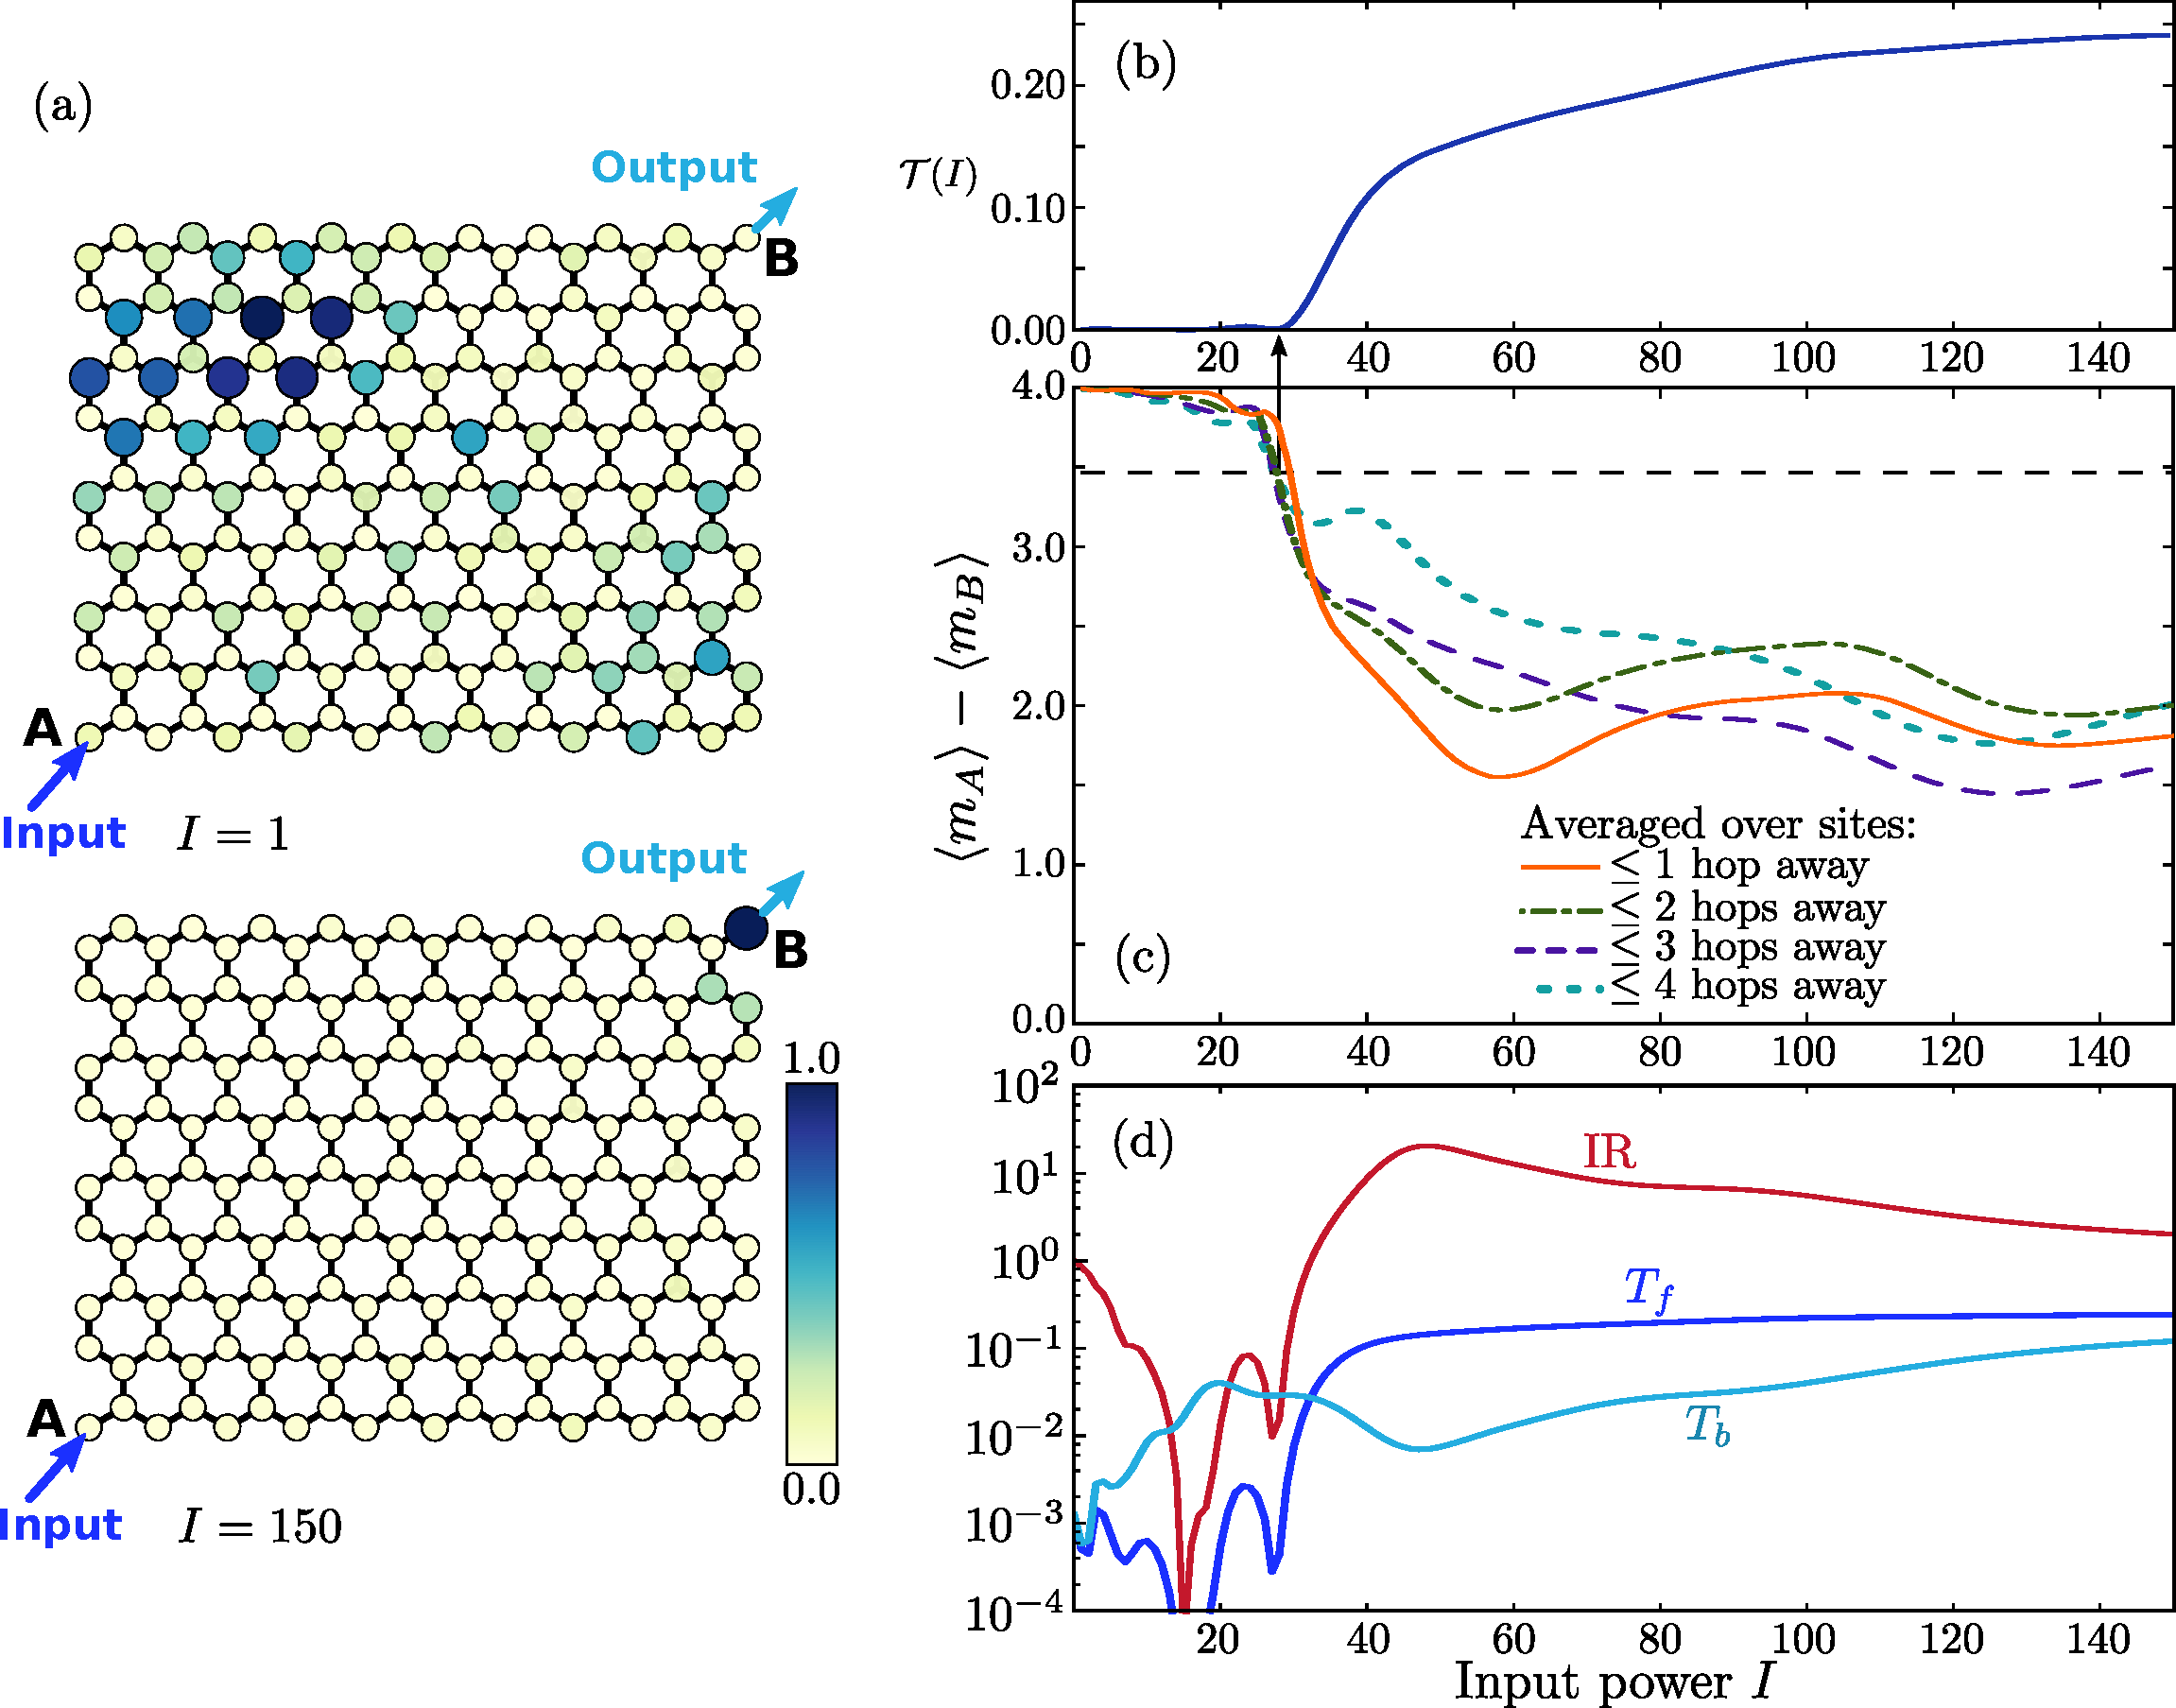
\includegraphics[width=0.9\textwidth, height=0.8\textwidth]{/home/zhouxin/research/conference/presentation/mtheme/slides/haldane.pdf}\hspace*{-10.5em}
           \column{0.4\linewidth}

Z = 19.2, $\eta_A=\eta_B=1.0$
 \vskip -0.1cm
 \hspace*{-2em}
{\small 1.T(I) increase significantly when $<m_A>-<m_B>$ crosses $2\sqrt{3}$}
 \vskip 0.1cm
 \hspace*{-2em}
{\small 2.$<m_A>-<m_B> = 2\sqrt{3}$ indicates topological trnasition for underline linear lattice}
 \vskip 0.1cm
 \hspace*{-2em}
{\small 3.$T_b$ is pretty smaller comparing to $T_f$ in a broad range of I.}





         \end{columns}
         \end{block}

\end{frame}

\begin{frame}{Topological Optical Isolation}
         \vskip -1.cm

         \begin{block}{Nonlinear Coupled Ring Lattices}
         
       \begin{columns}
          \column{0.4\linewidth}
             %\centering
             \hspace*{0.5em}
             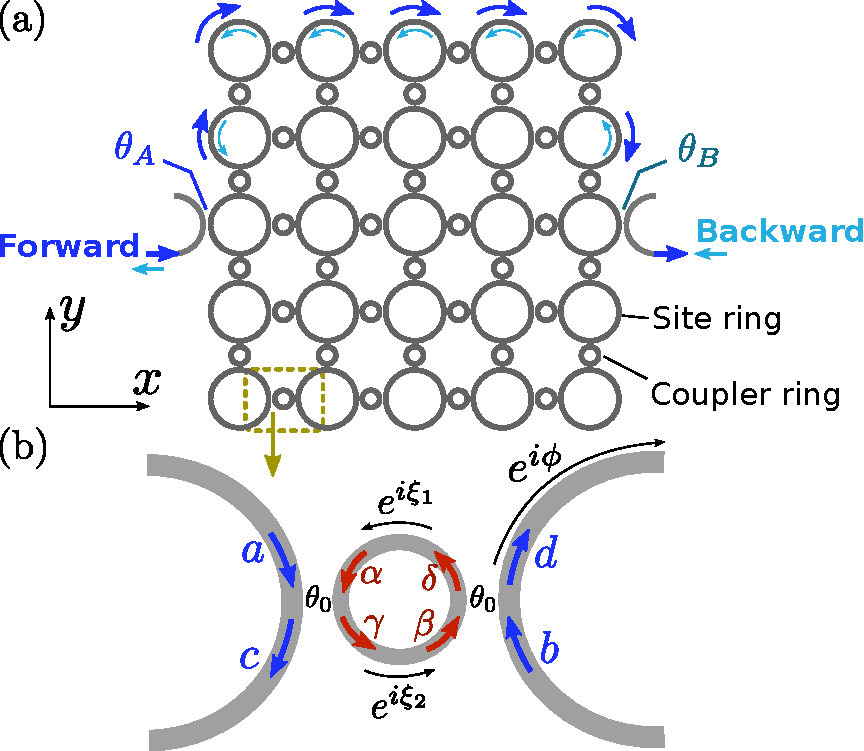
\includegraphics[width=0.9\textwidth, height=0.8\textwidth]{/home/zhouxin/research/conference/presentation/mtheme/slides/Lattice.pdf}\hspace*{-10.5em}
           \column{0.4\linewidth}
 
            \hspace*{0.5em}
             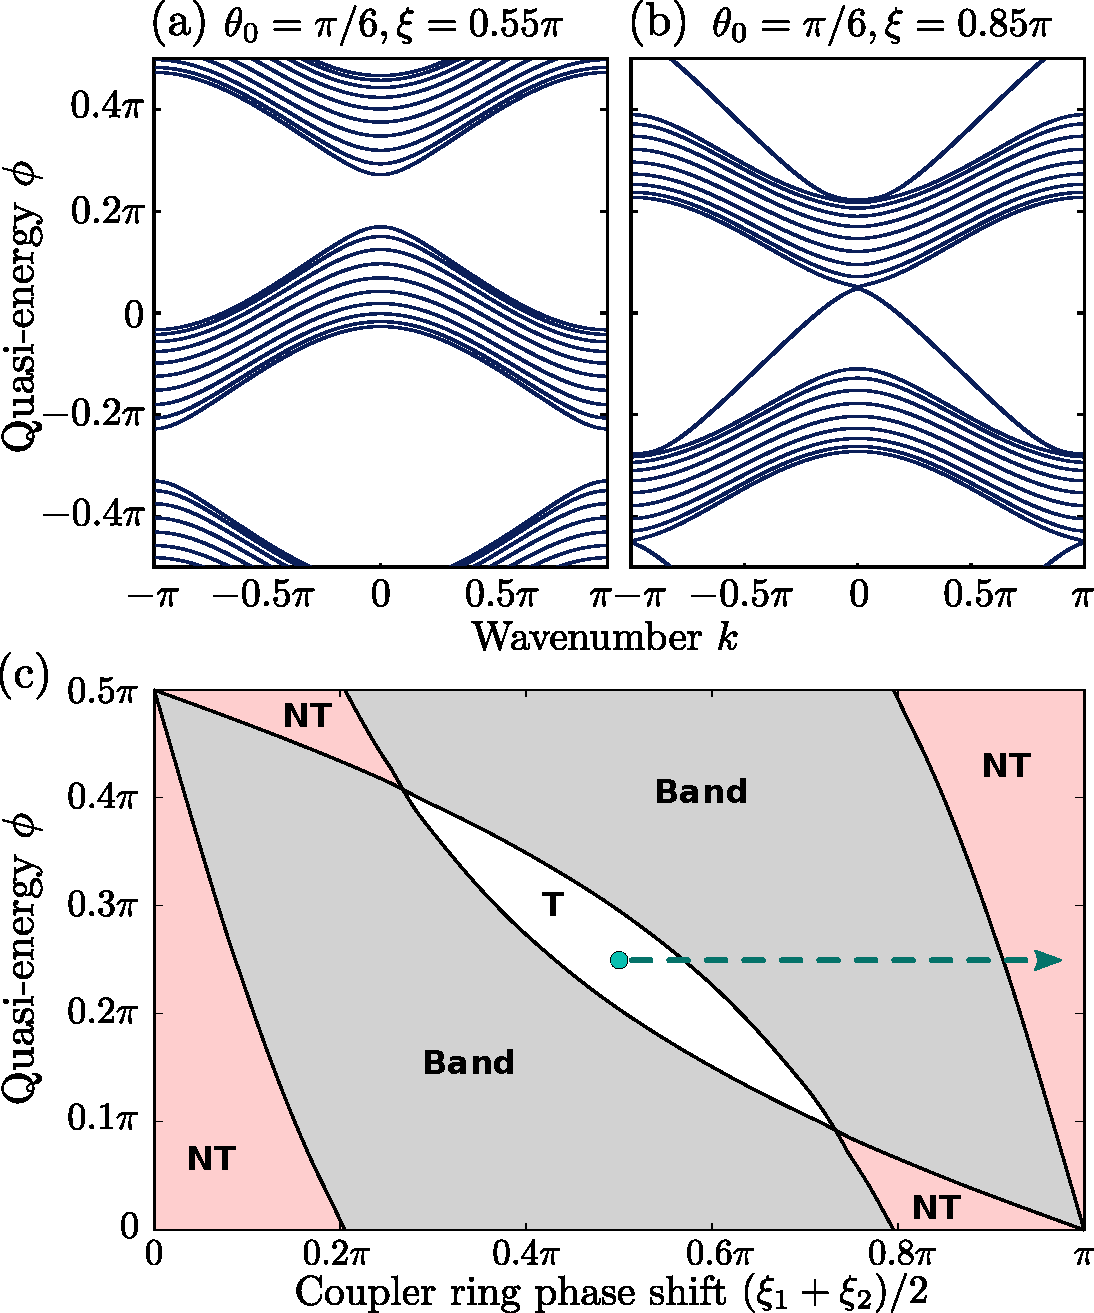
\includegraphics[width=0.9\textwidth, height=0.8\textwidth]{/home/zhouxin/research/conference/presentation/mtheme/slides/band_psi.pdf}\hspace*{-10.5em}





         \end{columns}
         \begin{eqnarray}
         \begin{bmatrix}
    c       \\
       \gamma  

\end{bmatrix}=S_c(\theta_0)\begin{bmatrix}
    a       \\
       \alpha  

\end{bmatrix}, \begin{bmatrix}
    d       \\
       \delta  

\end{bmatrix}=S_c(\theta_0)\begin{bmatrix}
    b       \\
       \beta  

\end{bmatrix}, S_c(\theta_0)=\begin{bmatrix}
    \sin(\theta_0) & i\cos(\theta_0)      \\
       i\cos(\theta_0) &  \sin(\theta_0)

\end{bmatrix}\\
\alpha = e^{i\xi_1}\delta, \beta = e^{i\xi_2}\gamma
         \end{eqnarray}
         \end{block}

\end{frame}


\begin{frame}{Topological Optical Isolation}
         \vskip -1.cm

         \begin{block}{Nonlinear Coupled Ring Lattices}
         Introduce Kerr-like nonlinearity to phase shift on each arm
         \begin{equation}
         \xi = \xi_0 + \kappa I        
         \end{equation}
       \begin{columns}
          \column{0.5\linewidth}
             %\centering
             \hspace*{0.5em}
             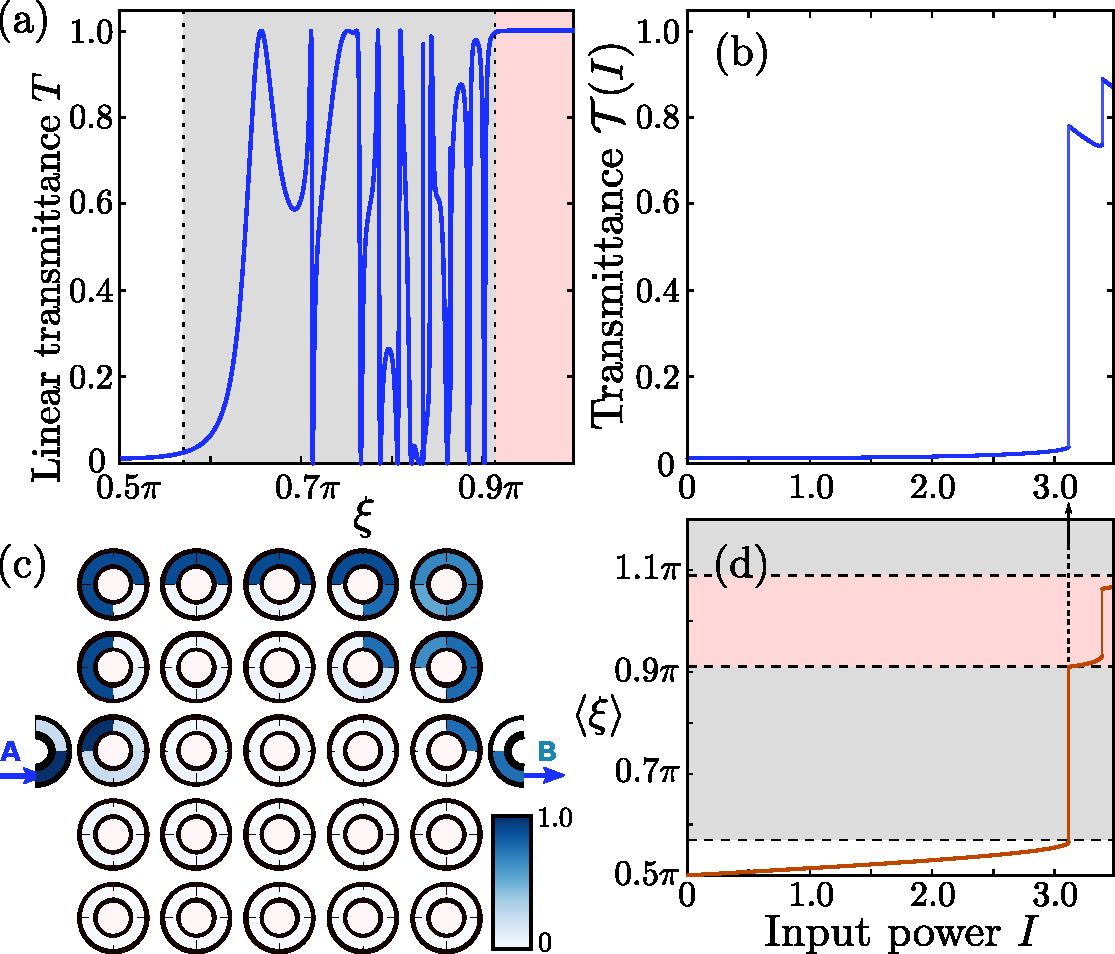
\includegraphics[width=0.9\textwidth, height=0.8\textwidth]{/home/zhouxin/research/conference/presentation/mtheme/slides/Trans_psi_1.pdf}\hspace*{-10.5em}
           \column{0.5\linewidth}
 
            \hspace*{0.5em}
             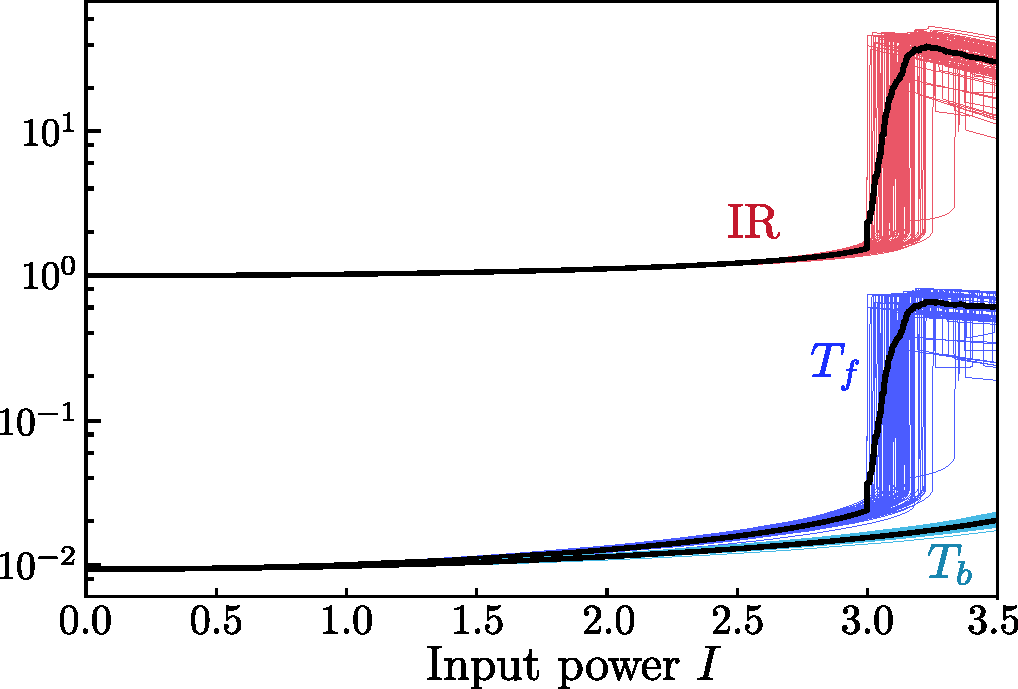
\includegraphics[width=0.9\textwidth, height=0.8\textwidth]{/home/zhouxin/research/conference/presentation/mtheme/slides/IRP2.pdf}\hspace*{-10.5em}





         \end{columns}

         \end{block}

\end{frame}
\begin{frame}{Conclusion}
         \vskip -1.cm

\end{frame}
\begin{frame}{Topological Photonics}
\begin{block}{Discover of Topological State}
Insulating in the bulk while conducting in the surface without backscattering even in the presence of impurities.
\begin{figure}
    \centering
    \begin{subfigure}[t]{0.4\textwidth}
        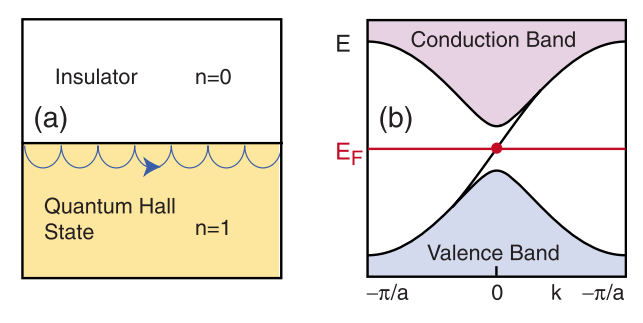
\includegraphics[width=\textwidth]{/home/zhouxin/research/conference/presentation/mtheme/slides/hall.png}
        \caption{Quantum Hall Effect. Time reversal symmetry is broken. Hasan and Kane, RMP, 2010}
        \label{fig:gull}
    \end{subfigure}\hspace*{3.0em}%
    ~ %add desired spacing between images, e. g. ~, \quad, \qquad, \hfill etc. 
      %(or a blank line to force the subfigure onto a new line)
    \begin{subfigure}[t]{0.415\textwidth}
        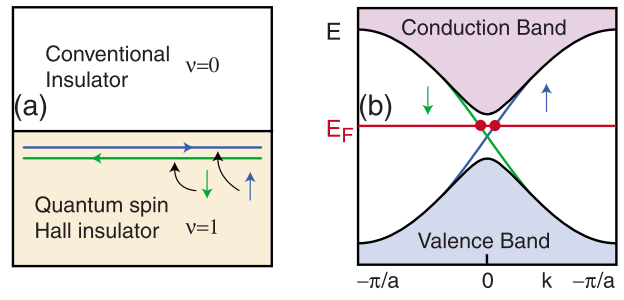
\includegraphics[width=\textwidth]{/home/zhouxin/research/conference/presentation/mtheme/slides/spin_hall.png}
        \caption{Quantum Spin Hall Effect. Time reversal symmetry is preserved. Hasan and Kane, RMP, 2010}
        \label{fig:tiger}
    \end{subfigure}
\label{fig:animals}
\end{figure}      

%\begin{variableblock}{Title}{bg=white}{bg=white}
%d
%\end{variableblock}

\end{block}

\end{frame}
\end{document}
